%%%%%%%%%%%%%%%%%%%%%%%%%%%%%%%%%%%%%%
%%%%%%%%%%%%%%%%%%%%%%%%%%%%%%%%%%%%%%
% Do not edit the TeX file your work
% will be overwritten.  Edit the RnW
% file instead.
%%%%%%%%%%%%%%%%%%%%%%%%%%%%%%%%%%%%%%
%%%%%%%%%%%%%%%%%%%%%%%%%%%%%%%%%%%%%%



Our final data analysis example is an application of a Bayesian topic model to
population genetics. We consider a publicly available dataset from
\citet{galbusera:2000:thrush} that contains genotypes from 155 individuals of an
endangered bird species, the Taita thrush. Individuals were collected from four
regions in southeast Kenya (Chawia, Mbololo, Ngangao, Yale), and each individual
was genotyped at seven micro-satellite loci. The four regions were once part of
a cohesive cloud forest that has since been fragmented by human development. For
this endangered bird species, understanding the degree to which populations have
grown genetically distinct is important for conservation efforts: well-separated
populations with little genetic diversity are particularly at risk of
extinction.  The goal of the analysis is to infer the population of origin for specific loci and estimate the degree to which populations are admixed in each
individual.


\subsubsection*{The model}

The data consists of consists of $\nindiv$ individuals genotyped at $\nloci$
loci. Let $\x_{\n\l\i}\in\{1, \ldots, J_\l\}$ be the observed genotype for
individual $\n$ at locus $\l$ and chromosome $\i$. $J_\l$ is the number of
possible genotypes at locus $\l$. For example, if the measurements are all
single nucleotides (A, T, C or G) then $J_\l = 4$ for all $\l$.

A latent population is characterized by the collection $\beta_k =
(\latentpop_{\k1}, \ldots, \latentpop_{\k\nloci})$ where
$\latentpop_{\k\l}\in\Delta^{J_\l - 1}$ are the latent frequencies for the $J_l$
possible genotypes at locus $\l$. Let $\z_{\n\l\i}$ be the assignment of
observation $\x_{\n\l\i}$ to a latent population. Notice that for a given
individual $\n$, different loci, or even different chromosomes at a given locus,
may have different population assignments. The distribution of
$\x_{\n\l\i}\in\{1, \ldots, J_\l\}$ arising from population $\k$ is
%
\begin{align*}
\p(\x_{\n\l\i} \vert \latentpop_{\k}) =
\categoricaldist{\x_{\n\l\i}\vert \latentpop_{\k\l}}.
\end{align*}

Unlike the previous models, we now have a stick-breaking process for each
individual. Draw sticks
%
\begin{align*}
\nu_{\n\k} \iid \pstick(\nu_{\n\k}) \quad \forall \n = 1, \ldots, \nindiv; \k = 1, 2, \ldots \infty.
\end{align*}
%
The prior assignment probability vector $\latentadmix_{\n} =
(\latentadmix_{\n1}, \latentadmix_{\n2}, \ldots)$, now unique to each
individual, is formed by the same stick-breaking construction as before,
%
\begin{align*}
\latentadmix_{\n\k} = \nu_{\n\k} \prod_{\k' < \k} (1 - \nu_{\n\k'}).
\end{align*}
%
The population assignment $\z_{\n\l\i}$ is drawn from the usual multinomial
distribution
%
\begin{align*}
p(\z_{\n\l\i} | \latentadmix_\n) = \prod_{k=1}^{\infty} \latentadmix_{\n\k}^{\z_{\n\l\i\k}}.
\end{align*}
%
In this genetics application, we call $\latentadmix_{\n}$ the \textit{admixture}
of individual $\n$.

This model is identical to fastSTRUCTURE, a model proposed in
\citet{pritchard:2000:structure, raj:2014:faststructure}, except that we replace
the Dirichlet prior in fastSTRUCTURE with an infinite stick-breaking process.
The result is a model similar to a hierarchical Dirichlet process for topic
modeling \citep{teh:2006:hdp}, but without the top-level Dirichlet process. In
addition, genotypes at genetic markers take the place of words in a document; in
lieu of inferring ``topics," we infer latent populations.

The variational approximation is mean-field as before, and all distributions are
conditionally conjugate except for the stick-breaking proportions, which remain
logit-normal. See \appref{app_structure} for further details.



\begin{knitrout}
\definecolor{shadecolor}{rgb}{0.969, 0.969, 0.969}\color{fgcolor}\begin{figure}[!h]

{\centering 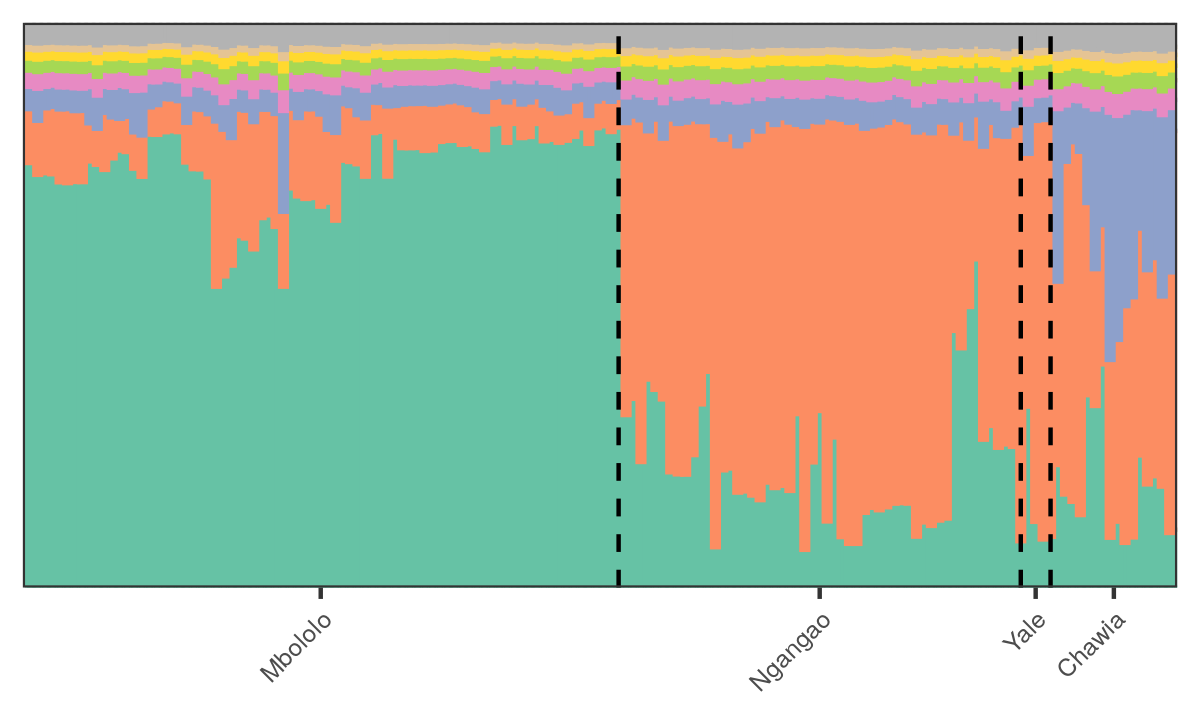
\includegraphics[width=0.980\linewidth,height=0.470\linewidth]{figure/stru_init_fit-1} 

}

\caption[The inferred individual admixtures at $\alpha_0 = 3$.
    Each vertical strip is an individual and each color
    a latent population.
    Lengths of colored segments represent the inferred admixture proportions.
    Individuals are ordered by the geographic region from which they were sampled
    (Mbololo, Ngangao, Yale, and Chawia).
    In the text, we refer to the green, orange, and purple latent populations
    as population 1, 2, and 3, respectively]{The inferred individual admixtures at $\alpha_0 = 3$.
    Each vertical strip is an individual and each color
    a latent population.
    Lengths of colored segments represent the inferred admixture proportions.
    Individuals are ordered by the geographic region from which they were sampled
    (Mbololo, Ngangao, Yale, and Chawia).
    In the text, we refer to the green, orange, and purple latent populations
    as population 1, 2, and 3, respectively. }\label{fig:stru_init_fit}
\end{figure}


\end{knitrout}

\subsubsection*{Quantity of interest}

The posterior quantities of interest in this application
are the admixtures $\pi_\n$. 
\figref{stru_init_fit} plots the inferred admixtures
$\expect{\q}{\pi_\n}$ for all individuals $\n$. 
The approximate posterior $\q$ was fit to a model with a
GEM prior at parameter $\alpha_0 = 3$.  
The choice of $\alpha_0 = 3$ corresponds to roughly four distinct populations 
{\em a priori} (\eqref{prior_num_clusters}), 
motivated by the fact that the individuals come from four geographic regions. 
Below, we will evaluate sensitivity to this prior choice. 

In the approximate posterior at $\alpha_0$, there
appear to be three dominant latent populations, which we arbitrarily label as
populations 1, 2, and 3 (\figref{stru_init_fit}). 
The inferred admixture proportions generally correspond with geographic regions:
Mbololo individuals are primarily population 1; 
Ngangao individuals are primarily population 2; 
and Chawia individuals are a mixture of populations 1, 2, and 3. 

Notably, outlying admixtures among individuals from the same geographic region provide clues into the historical migration patterns of this species.
For example,
while most Mbololo individuals are dominantly population 1,
several Mbololo individuals have abnormally 
large admixture proportions of population 2.
Conversely, while most Ngangao individuals are dominantly population 2, 
several Ngangao individuals have abnormally large admixture
proportions of population 1. This suggests that some migration has occurred
between the Mbololo and Ngangao regions.

We evaluate the sensitivity of this conclusion to possible prior perturbations.
Define the posterior quantity of interest
%
\begin{align*}
\gadmix(\eta; \mathcal{N}, k) =
 \expect{\q(\pi\vert\eta)}{\frac{1}{|\mathcal{N}|}\sum_{n\in\mathcal{N}}
\pi_{\n\k}},
\end{align*}
%
the average admixture proportion of population $\k$ in a set of
individuals $\mathcal{N}$.

Below, we consider $\gadmix$ with three different sets of individuals: 
$\mathcal{N} = \{26, ..., 31\}$, corresponding to 
the outlying Mbololo individuals, labeled 
``A" in \figref{stru_func_sens}; 
$\mathcal{N} = \{125, ..., 128\}$, corresponding to the four 
outlying Ngangao individuals, labeled ``B";
and $\mathcal{N} = \{139, ..., 155\}$ corresponding to all Chawia individuals, 
labeled ``C".
For individuals A, we let $\k=2$ in $\gadmix$ and 
examine the robustness of the presence of population 2; 
for individuals B, we use $\k = 1$; 
and for individuals C, we use $\k = 3$. 
The first two posterior quantities relate to the inferred migration between
the Mbololo and Ngangao regions. 
In the last example, we study the robustness of having a third latent
population present, a population which primarily appears in Chawia individuals.

\subsubsection*{Functional sensitivity}

We construct the worst-case negative perturbation
for decreasing each of our three variants of $\gadmix$, in order to see
whether the biologically interesting patterns can be made to disappear
with different prior choices.
\figref{stru_func_sens} shows the result of the worst-case perturbations 
on the prior density and $\gadmix$. 
After the worst-case perturbation, 
the admixture proportion of population 2 in individuals A 
was nearly halved.
On the other hand, the admixture of population 1 in individuals B 
is more robust.
We conclude that the inferred migration from Ngangao to
Mbololo is relatively robust to the stick-breaking prior, while 
conclusions about migration from Mbololo to Ngangao may be dependent on prior choices.




\begin{knitrout}
\definecolor{shadecolor}{rgb}{0.969, 0.969, 0.969}\color{fgcolor}\begin{figure}[!h]

{\centering 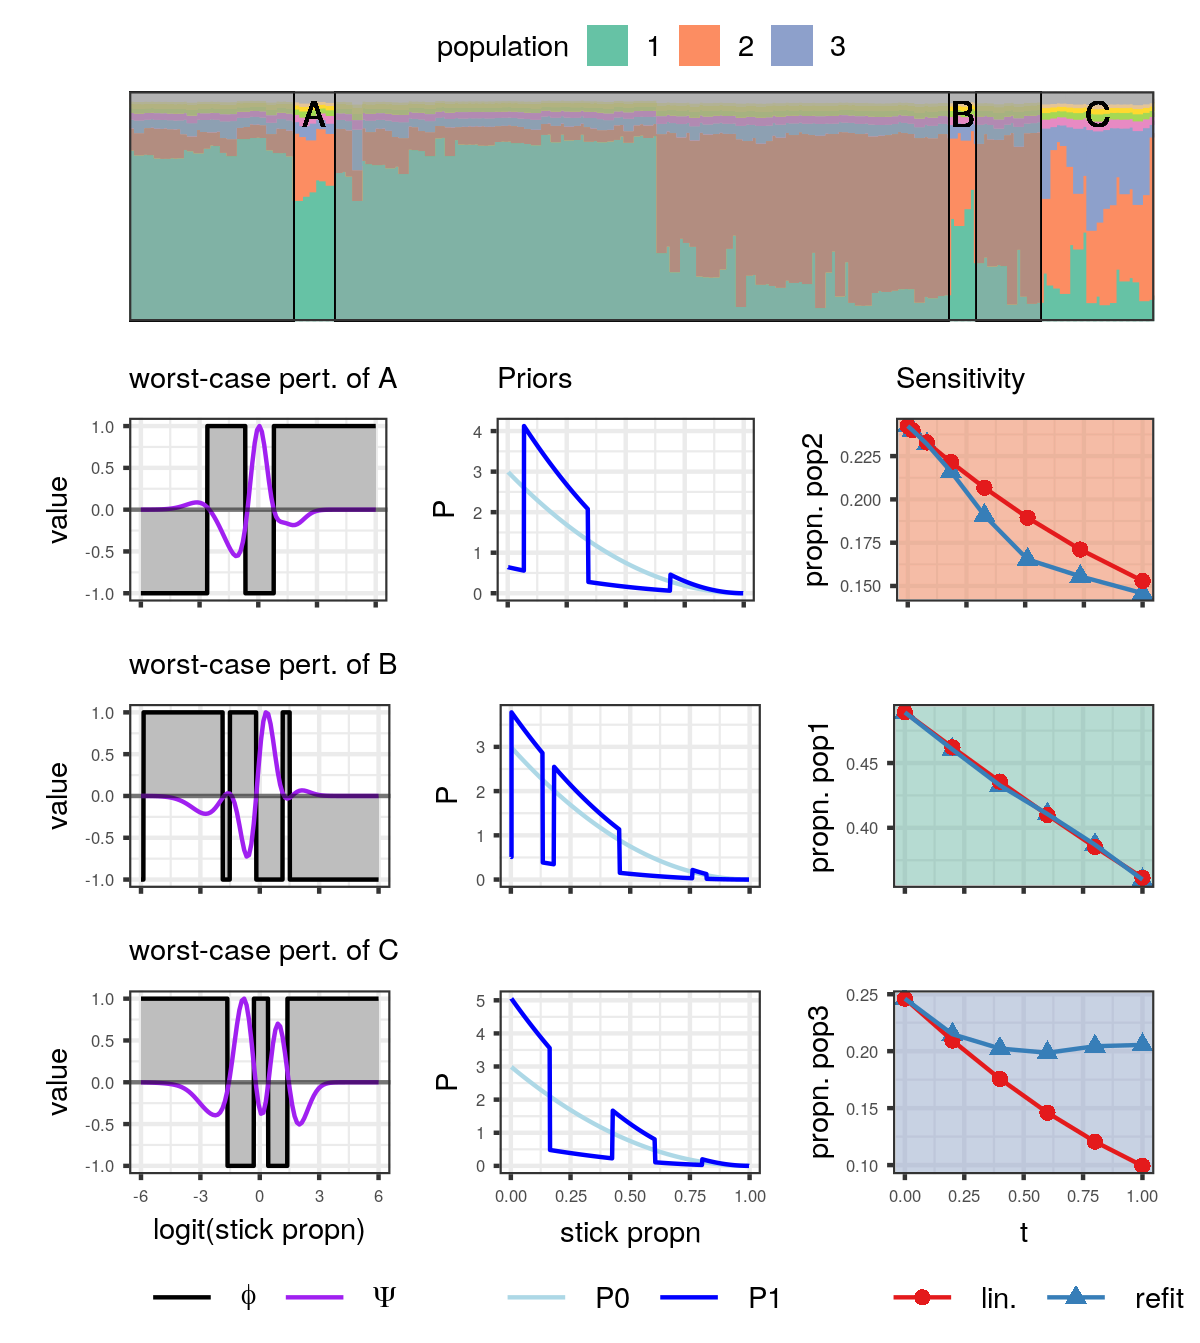
\includegraphics[width=0.980\linewidth,height=1.098\linewidth]{figure/stru_func_sens-1} 

}

\caption[Sensitivity of inferred admixtures for several outlying individuals.
     For individuals A,
     we examine the sensitivity of the admixture proportion of population 2.
     For individuals B,
     we examine the population 1 admixture
     For the individuals C, we examine the population 3 admixture.
     (Left column) The worst-case negative perturbation with
     $\norminf{\phi} = 1$
     in grey,
     plotted against the influence function in purple
     (scaled such that $\norminf{\psi} = 1$).
    (Middle column) The effect of the perturbation on the prior density.
    (Right column) Effects on the inferred admixture]{Sensitivity of inferred admixtures for several outlying individuals.
     For individuals A,
     we examine the sensitivity of the admixture proportion of population 2.
     For individuals B,
     we examine the population 1 admixture
     For the individuals C, we examine the population 3 admixture.
     (Left column) The worst-case negative perturbation with
     $\norminf{\phi} = 1$
     in grey,
     plotted against the influence function in purple
     (scaled such that $\norminf{\psi} = 1$).
    (Middle column) The effect of the perturbation on the prior density.
    (Right column) Effects on the inferred admixture. }\label{fig:stru_func_sens}
\end{figure}


\end{knitrout}



The conclusions from the linear approximation did not
always agree with the conclusions from refitting the
variational approximation 
in this data set and model. 
For example, the admixture proportion of population 3 in individuals C were predicted to more sensitive by our linear approximation than 
were actually observed after refitting (bottom row \figref{stru_func_sens}). 

Moreover, even though the linear approximation
agreed with the refits for individuals A in 
overall admixture proportion 
(\figref{stru_func_sens} second row),
the approximation does does not perform uniformly well over all individuals.
\figref{stru_func_sens_admix} plots the inferred admixtures
computed using the linearized variational parameters 
and the refitted variational parameters 
after the worst-case prior perturbation. 
The admixture proportion of population 2 in individual $n = 25$
dramatically increased after refitting with the perturbed prior;
the linearized parameters failed to reproduce this change.

Even though linear approximation works less well in this example, 
the influence function is still able to guide our choice of
functional perturbations at which to refit.
While the worst-case perturbations we used 
may be an adversarial choice, 
the influence function suggests that 
we can construct a smoother perturbation 
with a similar effect as the worst-case, 
as we did in \secref{results_mice}. 
Importantly, as we will note in the next subsection, 
the influence function is cheap to compute relative to refitting. 
For a more further discussion of the limitations of the linear approximation, 
see \appref{app_structure_results}.



\begin{knitrout}
\definecolor{shadecolor}{rgb}{0.969, 0.969, 0.969}\color{fgcolor}\begin{figure}[!h]

{\centering 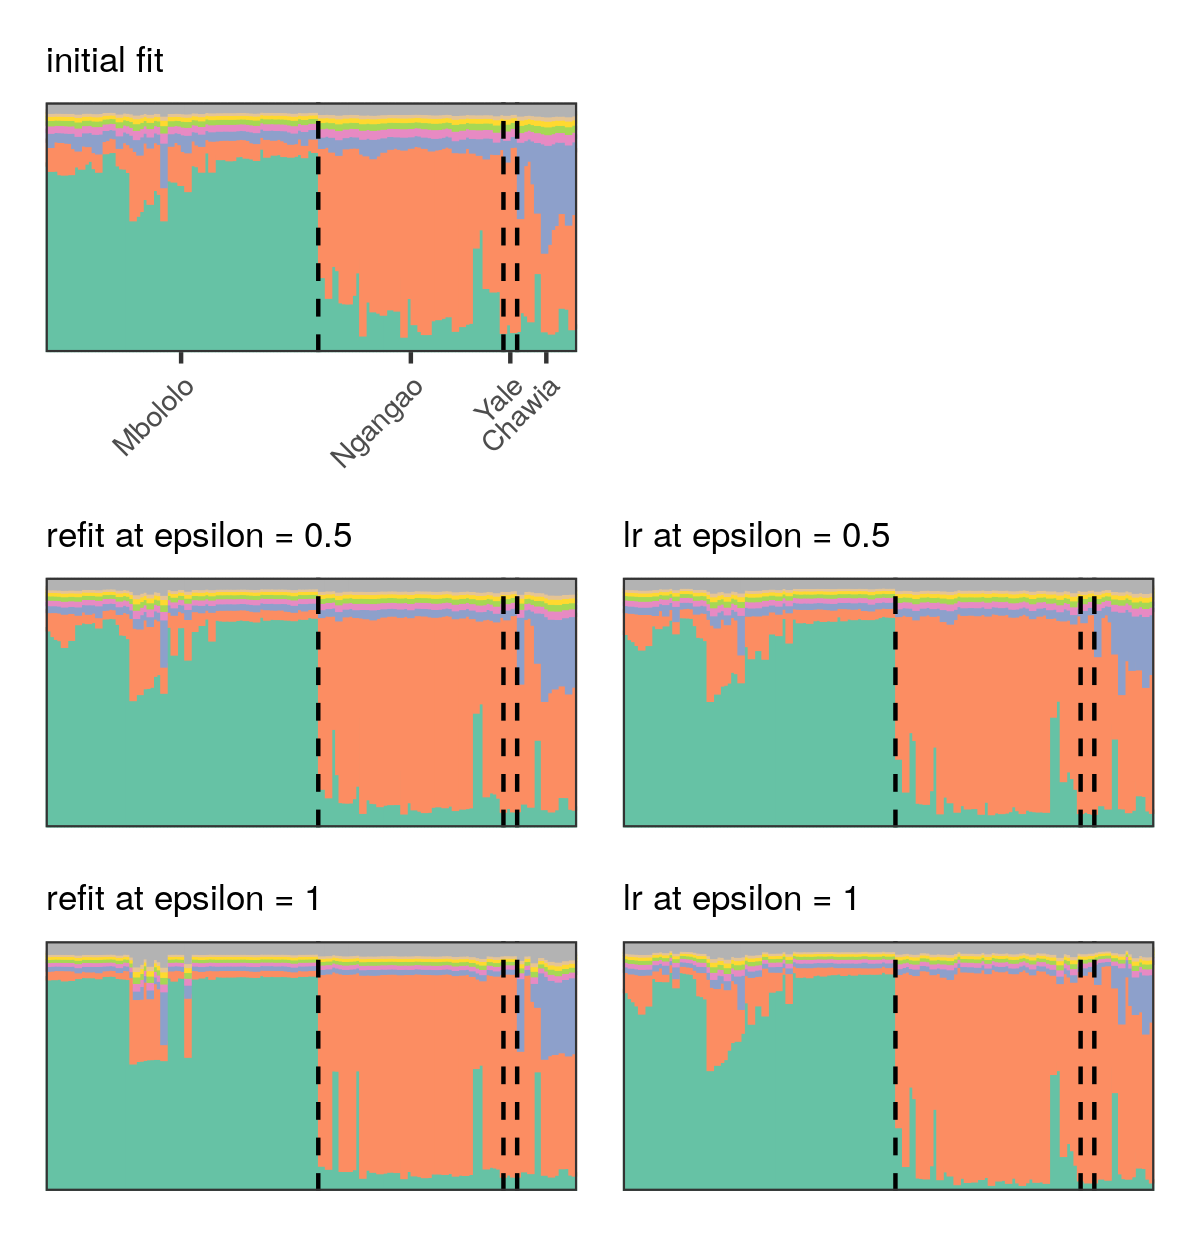
\includegraphics[width=0.980\linewidth,height=0.392\linewidth]{figure/stru_func_sens_admix-1} 

}

\caption{Inferred admixtures after the worst-case perturbation
     to individuals ``A" (see Figure~\ref{fig:stru_func_sens} for perturbation). }\label{fig:stru_func_sens_admix}
\end{figure}


\end{knitrout}


\newcommand{\StructureLimitationsA}{

\begin{knitrout}
\definecolor{shadecolor}{rgb}{0.969, 0.969, 0.969}\color{fgcolor}\begin{figure}[!h]

{\centering 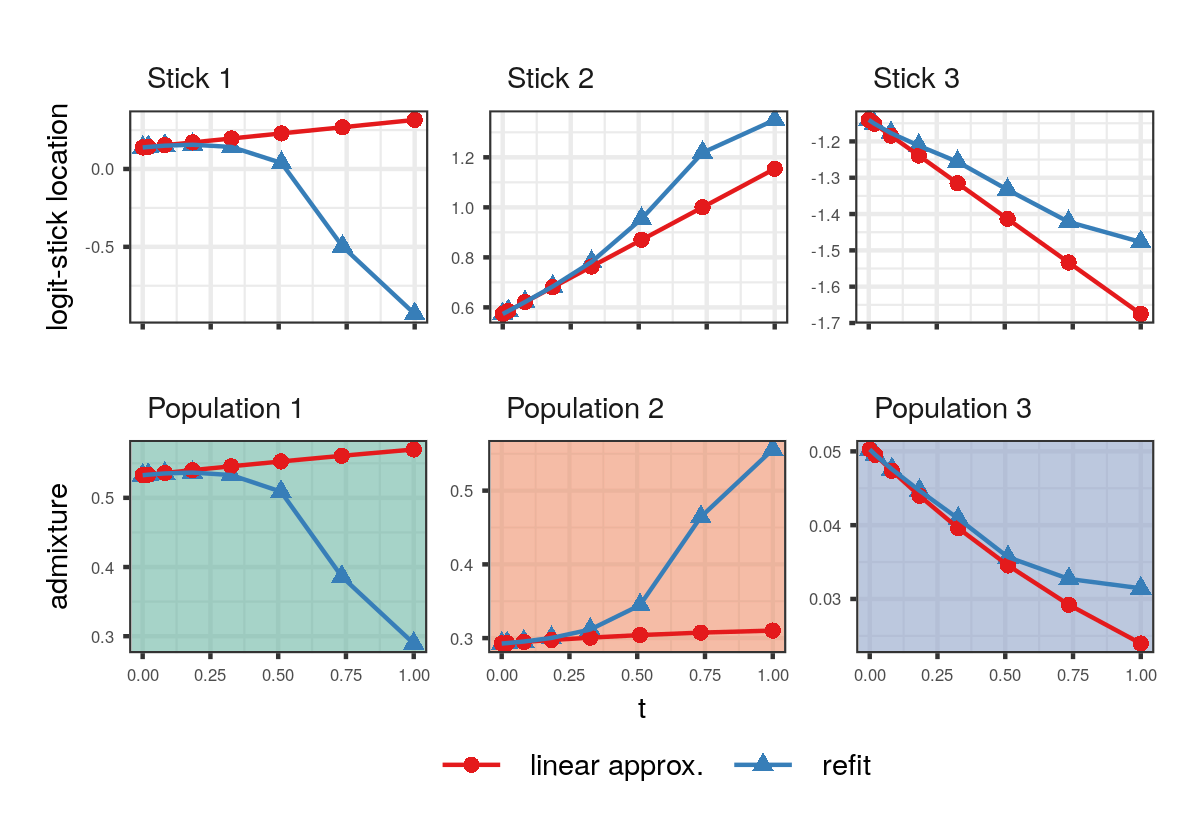
\includegraphics[width=0.980\linewidth,height=0.666\linewidth]{figure/stru_lin_bad_example-1} 

}

\caption[An individual $(\n = 26)$ for which
    the linearly approximated variational parameters
    poorly captured the
    change in admixture observed after refitting
    as $\t \rightarrow 1$.
    (Top row) the change in location parameter of the normally
    distributed logit-sticks, for the first three sticks.
    The response here is a variational parameter, so
    the approximation (red) is necessarily linear with respect to $\t$.
    (Bottom row) the change in the inferred admixtures for
    populations 1, 2, and 3]{An individual $(\n = 26)$ for which
    the linearly approximated variational parameters
    poorly captured the
    change in admixture observed after refitting
    as $\t \rightarrow 1$.
    (Top row) the change in location parameter of the normally
    distributed logit-sticks, for the first three sticks.
    The response here is a variational parameter, so
    the approximation (red) is necessarily linear with respect to $\t$.
    (Bottom row) the change in the inferred admixtures for
    populations 1, 2, and 3. }\label{fig:stru_lin_bad_example}
\end{figure}


\end{knitrout}
}

\newcommand{\StructureLimitationsB}{

\begin{knitrout}
\definecolor{shadecolor}{rgb}{0.969, 0.969, 0.969}\color{fgcolor}\begin{figure}[!h]

{\centering 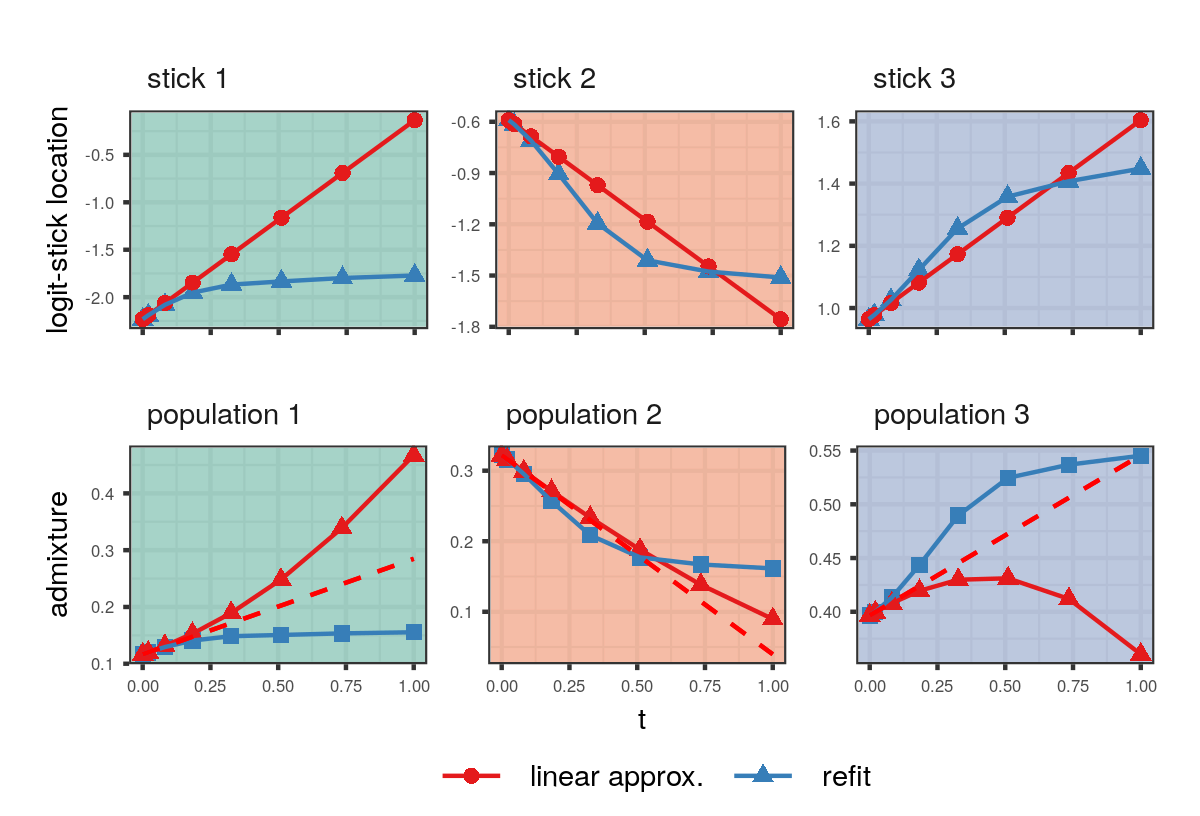
\includegraphics[width=0.980\linewidth,height=0.666\linewidth]{figure/stru_fully_lin_example-1} 

}

\caption[An example where
    linearizing the posterior quantity itself outperforms
    linearizing the variational parameters only.
    Shown are logit-stick location parameters (top row) and
    inferred admixtures (bottom row)
    for individual $n = 74$ and populations $k = 1, 2$ and $3$.
    Dashed red is the approximation $\glin(\t)$ formed by linearizing the
    inferred admixture $\expect{\q}{\pi_{\n\k}}$ with respect to prior
    parameter $t$.
    On the admixture proportion of population 3,
    $\glin(\t)$ outperforms $\g(\etalin(\t))$ (solid red)]{An example where
    linearizing the posterior quantity itself outperforms
    linearizing the variational parameters only.
    Shown are logit-stick location parameters (top row) and
    inferred admixtures (bottom row)
    for individual $n = 74$ and populations $k = 1, 2$ and $3$.
    Dashed red is the approximation $\glin(\t)$ formed by linearizing the
    inferred admixture $\expect{\q}{\pi_{\n\k}}$ with respect to prior
    parameter $t$.
    On the admixture proportion of population 3,
    $\glin(\t)$ outperforms $\g(\etalin(\t))$ (solid red). }\label{fig:stru_fully_lin_example}
\end{figure}


\end{knitrout}
}
